The $\wenuplusjets$ process enters the signal region, thus contributing to the
background, in case the electron is not identified in the detector. In the
$\wtaunuplusjets$ process the $\tau$ particle can decay hadronically in 65\% of
the cases resulting in additional jets that can help this background mimic the
signal. To address these backgrounds an electron control region
(CR$_\mathrm{\, ele}$) is built. It is designed to constrain both
$\wenuplusjets$ and $\wtaunuplusjets$ processes thanks to the decays of $\tau$
leptons into electrons. In order to efficiently reject the multi-jet background,
the electron is retained in the $\met$ calculation, the missing transverse
momentum in this case measures the momentum of the escaping neutrino. In
addition to cuts from A to H defined in \cref{sec:event-selection} the
CR$_\mathrm{\, ele}$ region selects events with:
\begin{itemize}
\item Exactly one good electron.
\item No additional baseline electrons or baseline muons in the final state.
\end{itemize}
In order to enhance the $\wtaunuplusjets$ contribution in this region, no
$m_\mathrm{\, T}$ cut is applied.
\cref{fig:ele_cr_plots}
% \cref{fig:ele_cr_et_miss_pre_fit,fig:ele_cr_jet1_pt_pre_fit}
shows the observed and predicted $\met$ and the leading jet $\pt$ distribution
in this control region. The overall agreement between data and MC is good and
improved after the global likelihood fit procedure described in
\cref{sec:glob-simult-likel}.
% \begin{figure}[!htb]
%   \centering
%   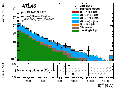
\includegraphics[width=.8\linewidth]{ele_cr_et_miss_post_fit}
%   \caption{Observed and predicted $\met$ distribution after the background only
%     fit in the electron $\crele$ for the $\met > 250~$GeV selection. The error
%     bands include the statistical and systematic errors.}
%   \label{fig:ele_cr_et_miss_pre_fit}
% \end{figure}
% \begin{figure}[!htb]
%   \centering
%   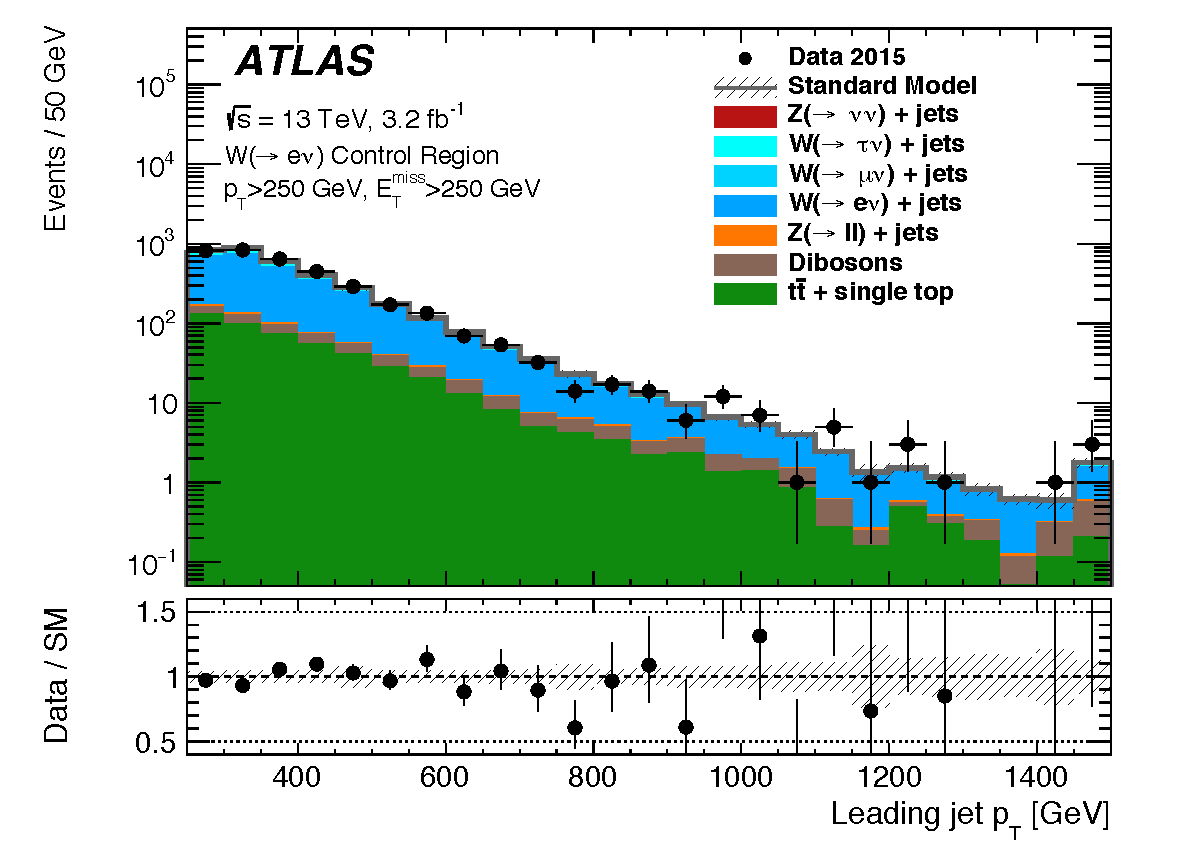
\includegraphics[width=.8\linewidth]{ele_cr_jet1_pt_post_fit}
%   \caption{Observed and predicted $\pt$ distribution after the background only
%     fit in the electron $\crele$ for the $\met > 250~$GeV selection. The error
%     bands include the statistical and systematic errors.}
%   \label{fig:ele_cr_jet1_pt_pre_fit}
% \end{figure}
\begin{figure}[!htb]
  \centering
  \begin{subfigure}[t]{.48\linewidth}
    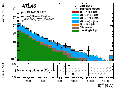
\includegraphics[width=\linewidth]{ele_cr_et_miss_post_fit}
    \caption{$\met$ distribution.}
    \label{fig:ele_cr_et_miss_pre_fit}
  \end{subfigure}
  \begin{subfigure}[t]{.48\linewidth}
    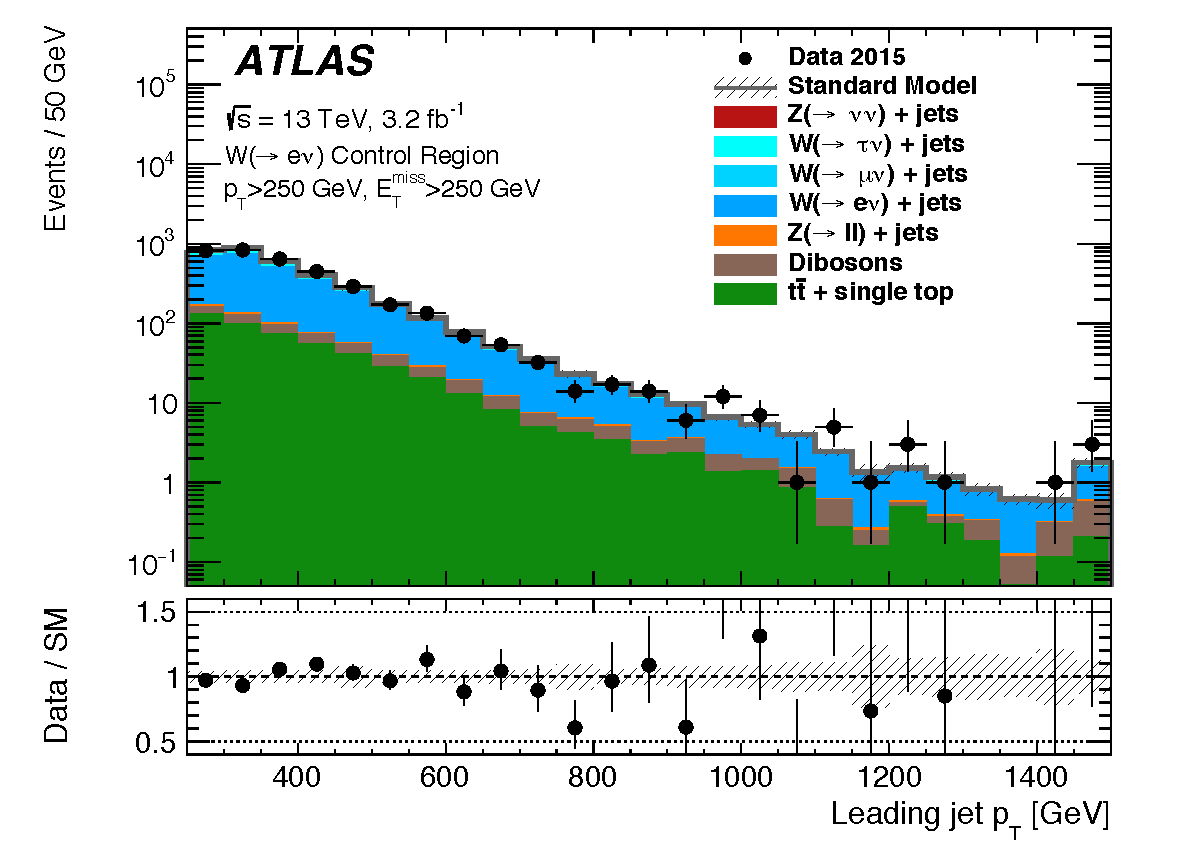
\includegraphics[width=\linewidth]{ele_cr_jet1_pt_post_fit}
    \caption{Leading jet $\pt$ distribution.}
    \label{fig:ele_cr_jet1_pt_pre_fit}
  \end{subfigure}
  \caption{Observed and predicted $\met$ and leading jet $\pt$ distributions
    after the background only fit in the electron $\crele$ for the
    $\met > 250~$GeV selection. The error bands include the statistical and
    systematic errors.}
  \label{fig:ele_cr_plots}
\end{figure}
%%% Local Variables:
%%% mode: latex
%%% TeX-master: "../search_for_DM_LED_with_ATLAS"
%%% End:
